\documentclass[ebook]{sigproc}

\directlua{
  if os.env["MODE"] == "production" then else
    tex.sprint("\\usepackage[colorspec=0.9]{draftwatermark}")
  end
}

\usepackage{graphicx,xcolor}
\usepackage[unicode,pdfusetitle]{hyperref}
\usepackage{xr,subfiles}
\usepackage{pdfpages}
\usepackage{makeidx}
\usepackage{comment}

% style/ 以下のスタイルファイル
\usepackage{sigproc-base}
\usepackage{sigproc-math}

% 各種パッケージの初期設定
\title{信号解析の数理}
\author{calamari-dev}
\date{\today}
\hypersetup{
  pdfsubject={線型代数で信号を理解するために},
  pdfkeywords={線型代数,関数解析,時間周波数解析,信号処理},
  colorlinks=true,
  allcolors=blue
}
\externaldocument[xr-]{\subfix{main}}
\makeindex

\begin{document}
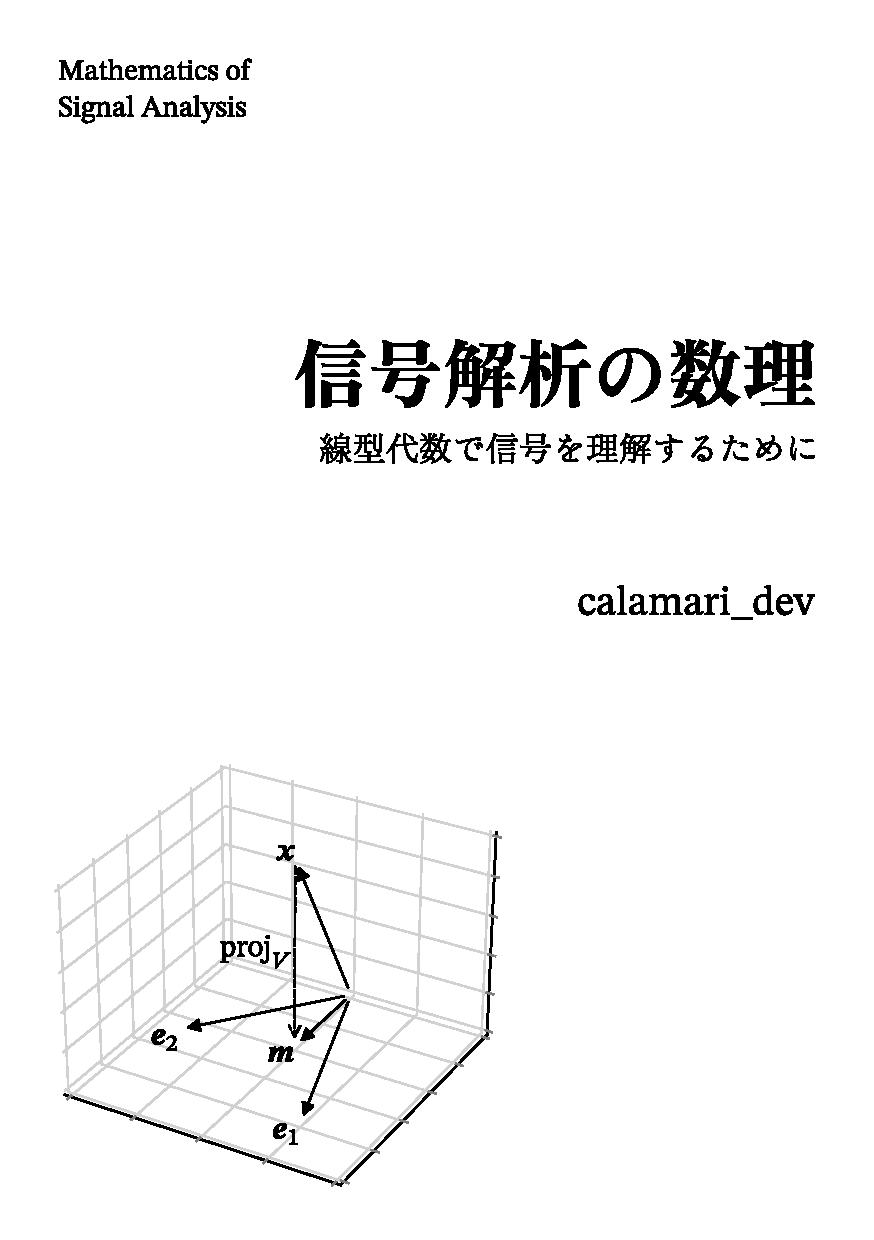
\includepdf{titlepage/titlepage.pdf}

\frontmatter
\subfile{chapter/getting_started/index}

\tableofcontents

\subfile{chapter/symbols/index}

\mainmatter
\subfile{chapter/numerical_vector_space/index}

\subfile{chapter/hilbert_space/index}

\subfile{chapter/probability_space/index}

\appendix
\subfile{chapter/program_example/index}

\backmatter
\subfile{chapter/references/index}

\printindex

\end{document}
